%%%% paper/ral_v1.tex -- IEEE Robotics and Automation Letters version (2026-11-05), supersedes draft_v1.tex (IJCAI).
%%%% Limit: 6 pages incl. references (+2 paid). Single-blind (RA-L): author block is a placeholder for the PI.
%%%%
%%%% Number policy (unchanged from draft_v1): every number is copied from a repo file; "% SRC:" names it.
%%%% Headline Config G numbers + Table I are GENERATED (viz/paper_numbers.py -> gen/numbers.tex, gen/table_crossover.tex)
%%%% and Fig. 1 by viz/paper_figures.py: from the amend39 re-run (settled 5 s + 0.30 m band, prereg amend39 + addendum 1)
%%%% when it exists, otherwise from the registered @T reports with a dagger. Re-run both scripts after amend39; the
%%%% \ifpending switch flips the dependent sentences. Config S numbers: results/amend39_configS_band/report.json (b=0.30)
%%%% and results/amend38_settled_recompute/report.json (b=0).
%%%% Hand-typed @T numbers that amend39 stages C/D will replace carry a manual \dag (margin, gate, Config G layer split).

\documentclass[letterpaper,10pt,journal,twoside]{IEEEtran}

\usepackage{cite}
\usepackage{amsmath,amssymb}
\usepackage{graphicx}
\usepackage{booktabs}
\usepackage{multirow}
\usepackage{url}
\usepackage[hidelinks]{hyperref}

\graphicspath{{figs/}}

\newcommand{\Tf}{T_{\mathrm{frame}}}
\newcommand{\tslot}{t_{\mathrm{slot}}}
\newcommand{\dsafe}{d_{\mathrm{safe}}}
\newcommand{\ci}[2]{\,[#1,\,#2]}
% GENERATED by viz/paper_numbers.py (source: legacy) -- do not edit
\newif\ifpending
\pendingtrue
\newcommand{\HeadMetric}{safe success at $T$}
\newcommand{\HeadShort}{safe@$T$}
\newcommand{\Pending}{\textsuperscript{\dag}}
\newcommand{\PendingNote}{\textsuperscript{\dag}Scored at the final instant $T$ (registered metric); being re-run under the settled metric with archived trajectories (prereg.\ amend39).}
\newcommand{\GapFifty}{$+0.936\ci{+0.912}{+0.960}$}
\newcommand{\RecFifty}{99}
\newcommand{\GapHundred}{$+0.880\ci{+0.848}{+0.908}$}
\newcommand{\RecHundred}{88}
\newcommand{\GapOneFifty}{$+0.479\ci{+0.445}{+0.511}$}
\newcommand{\RecOneFifty}{48}
\newcommand{\GapTwoHundred}{$+0.137\ci{+0.121}{+0.154}$}
\newcommand{\RecTwoHundred}{14}
\newcommand{\TauLearned}{0.986 / 0.892 / 0.545 / 0.178}
\newcommand{\TauGap}{$+0.986$, $+0.892$, $+0.545$, $+0.178$}
\newcommand{\TauEverFixed}{0.014 / 0.072 / 0.455 / 0.822}
\newcommand{\TauEverSweep}{0.008 / 0.076 / 0.473 / 0.827}
\newcommand{\TauComplFixed}{1.000 / 0.958 / 1.000 / 1.000}
\newcommand{\ComplLearnedLargeN}{0.857 / 0.599}
\newcommand{\NoiseHead}{1.000 / 1.000 / 1.000 / 1.000 / 0.968}
\newcommand{\Headroom}{$+0.120$ / $+0.521$ / $+0.831$}
\newcommand{\SafeNReal}{25}
\newcommand{\SafeNLearned}{50}


\markboth{IEEE Robotics and Automation Letters. Preprint version. Accepted Month, Year}%
{Staleness, Not Density: Where Delay Compensation Belongs in an MFG+CBF Swarm}

\begin{document}

\title{Staleness, Not Density, Limits Safety: Where Delay Compensation Belongs in a Mean-Field-Game Swarm with a Barrier Safety Filter}

\author{Author~One and Author~Two% <-- PI: names, affiliations, funding
\thanks{Manuscript received Month DD, YYYY; revised Month DD, YYYY.}%
\thanks{Affiliation and contact (to be completed).}}

\maketitle

\begin{abstract}
We study a decentralized drone swarm that routes with an offline mean-field-game (MFG) controller and
enforces separation with a per-agent control-barrier-function (CBF) safety filter. Agents sense neighbours
through noisy UWB range and vision bearing and exchange states over a TDMA channel whose frame grows linearly
with swarm size $N$, so a larger swarm acts on older information. In controlled simulation with a
drone-sized keep-out distance we find: (i)~collisions are caused by the \emph{staleness} of neighbour
estimates, not by density. With the delay removed but noise, packing and routing kept, no agent comes within
0.30\,m of another up to $N{=}200$, and a TDMA-slot sweep at fixed $N$ reproduces the collision rate of the
$N$-sweep at equal frame length. (ii)~Delay compensation must be fed to the CBF layer: given to the MFG
density term, even an oracle estimate changes safe success by exactly zero, while given to the CBF it
recovers the delay-free level. The MFG layer earns its place on liveness, $+0.35$ settled success over a
CBF-only swarm that deadlocks. A pooled-$N$ learned predictor recovers \RecHundred\% of the delay-induced
gap at $N{=}100$ and \RecTwoHundred\% at $N{=}200$\Pending. (iii)~A conformally calibrated per-neighbour
uncertainty margin does not beat a constant margin, and its coverage guarantee breaks in closed loop.
\end{abstract}

\begin{IEEEkeywords}
Swarm robotics, collision avoidance, multi-robot systems, robot safety, networked robots.
\end{IEEEkeywords}

%=====================================================================
\section{Introduction}
%=====================================================================
\IEEEPARstart{M}{ean-field-game} (MFG) controllers suit large swarms: each agent responds to a density
field rather than to every neighbour, and the equilibrium trades progress against
congestion~\cite{lasry2007mean,huang2006large,elamvazhuthi2019mean}. Deployed swarms add physics the
continuum model omits. Drones have a body size; neighbours are measured, not known (UWB ranging and camera
bearing are noisy); and neighbour states arrive over a shared radio. With time-division multiple access
(TDMA) each agent broadcasts once per frame, and the frame grows as $\Tf = N\tslot$. A CBF safety
filter~\cite{ames2017cbf,wang2017safety} is the standard way to add hard separation to such a controller,
but it is only as good as the neighbour positions it is given.

We ask a narrow design question for a two-layer MFG+CBF swarm: \emph{under realistic sensing and TDMA delay,
what limits safety, and where in the stack should delay compensation enter?} Our contributions are:
\begin{enumerate}
\item \textbf{An isolated mechanism for staleness-limited safety.} Removing only the delay removes every
  collision up to $N{=}200$; at fixed $N$, lengthening only the TDMA slot reproduces the collision rate of the
  $N$-sweep at equal $\Tf$ (Sec.~\ref{sec:barrier}).
\item \textbf{A separation of layer roles under delay.} Compensation fed to the MFG density term is worth
  exactly zero safety, even as an oracle; fed to the CBF it recovers the delay-free level. The MFG layer pays
  for itself in liveness (Sec.~\ref{sec:layers}).
\item \textbf{A negative result} for a calibrated uncertainty margin as a substitute for accurate
  compensation (Sec.~\ref{sec:sigma}).
\end{enumerate}
We also make the arrival metric explicit: success is scored as \emph{settled} arrival with a one-body
tolerance band, because scoring at the final instant rewards last-second inflow (Sec.~\ref{sec:metric}).

%=====================================================================
\section{Related Work}
%=====================================================================
\emph{MFGs for swarms.} MFGs couple a Hamilton--Jacobi--Bellman equation for a representative agent with a
Fokker--Planck equation for the population~\cite{lasry2007mean,huang2006large}, solved numerically by finite
differences~\cite{achdou2010mean}; mean-field models are widely used to design swarm
behaviour~\cite{elamvazhuthi2019mean}. They assume that the density an agent responds to is either the
equilibrium or a current local estimate; we study what happens when that estimate is built from stale, noisy
broadcasts.

\emph{CBFs for multi-agent safety.} CBF quadratic programs enforce forward invariance of a safe
set~\cite{ames2017cbf,ames2019cbf} and extend to multi-robot collision avoidance through decentralized pairwise
constraints~\cite{borrmann2015control,wang2017safety}. We use such a filter unchanged as the safety layer.

\emph{Measurement-robust and delay-aware CBFs.} Robust CBFs tighten the constraint by an error
bound~\cite{jankovic2018robust}; measurement-robust CBFs do so for learned
perception~\cite{dean2020guaranteeing,cosner2021measurement}; sampled-data and input-delay formulations treat
delay in the agent's own actuation loop~\cite{singletary2020sampled,molnar2023delay}. Closest to us, Ballotta
and Talak~\cite{ballotta2025safe} show that predicting neighbours' current states from delayed messages and
their age of information restores the safety of distributed CBF control. We take this predictor-into-CBF
mechanism as given. Our delay is set by the TDMA schedule, grows with $N$ and differs per neighbour, so a
worst-case bound is very conservative.

\emph{Stochastic and conformal safety.} Stochastic CBFs give probabilistic invariance under process
noise~\cite{clark2021stochastic}. Conformal prediction~\cite{vovk2005algorithmic,shafer2008tutorial,angelopoulos2023conformal}
yields distribution-free prediction regions and has been used to plan around predicted
agents~\cite{lindemann2023safe,dixit2023adaptive}. Its guarantee is marginal and assumes exchangeability between
calibration and deployment; Sec.~\ref{sec:sigma} is a concrete closed-loop instance of that caveat.

\emph{How we differ.} Our questions are about a \emph{hierarchical} controller: \emph{which layer} must receive
the compensation (answered by a layer-split ablation with a learned and an oracle estimate), whether the limit
is staleness or density (answered by a matched-staleness sweep), and whether a calibrated uncertainty margin can
replace accurate compensation. Classical compensators, constant-velocity extrapolation and a Smith-type model
predictor~\cite{smith1957closer}, are included as comparators.

%=====================================================================
\section{System Model and Protocol}
\label{sec:model}
%=====================================================================
\emph{Agents and task.} $N$ single-integrator agents ($\Delta t{=}0.01$\,s, speed clipped at 8\,m/s) cross a
wall through one gate and must reach a goal disc. Two agents collide when their true distance falls below
$D_{\mathrm{c}}{=}0.30$\,m, the body of a 5-inch quadrotor.
% SRC: experiments/amend21_cells/*.yaml (dt_exec 0.01); prereg/prereg_projectA.md Sec.3 (D_COLLISION 0.30, V_MAX 8.0)

\emph{Two-layer controller.} \emph{Macro:} an offline MFG equilibrium (fictitious play, Ces\`aro mean) is solved
once per scenario and $N$, giving a routing field $\Phi$ and equilibrium density $m^\star$. The nominal control is
\begin{equation}
u_i^{\mathrm{nom}} = -\nabla\Phi(x_i) - c_{\mathrm{d}}\nabla\big(\hat m_i - m^\star(x_i,t)\big)^2 + F_{\mathrm{bar}}(x_i;\hat x_{i\cdot}),
\end{equation}
where $\hat m_i$ is a kernel density estimate (bandwidth 0.60\,m, sensing radius 5\,m) built from agent $i$'s
\emph{estimates} $\hat x_{ij}$ of its neighbours and $F_{\mathrm{bar}}$ is a bounded soft barrier.
\emph{Micro:} each agent solves a CBF-QP that stays closest to $u_i^{\mathrm{nom}}$ subject to
$\|\hat x_{ij}-x_i\|\ge\dsafe$ for every sensed neighbour, with penalized slack so the QP is always feasible.
$\dsafe$ is the only safety knob. Both layers consume the same $\hat x_{ij}$ unless a layer-split ablation gives
each layer its own source.
% SRC: control/law.py; control/cbf.py; prereg/prereg_projectA.md Sec.2-3

\emph{Perception and TDMA.} Agent $j$ broadcasts once per frame in slot $j$, so $\Tf{=}N\tslot$ (nominal
$\tslot{=}5$\,ms) and the age of $i$'s information about $j$ is the sawtooth $(t-j\tslot)\bmod\Tf$. Each
broadcast yields a UWB range ($\sigma_r{=}0.10$\,m) and a bearing ($\sigma_\theta{=}0.035$\,rad).
The neighbour estimate is one of: \textbf{real} (stale and noisy, uncompensated); \textbf{noise\_only} (same noise
draws, age 0: perfect delay compensation); \textbf{fresh} (exact positions, oracle); \textbf{cv}
(constant velocity from the last two broadcasts); \textbf{smith} (propagation along $\Phi$); and \textbf{learned}
(Sec.~\ref{sec:method}).
% SRC: compensation/perception.py L27-32; control/params.py (SIGMA_THETA = radians(2)); review_amend24 B.1

\emph{Configurations.} \emph{Config~G} (scaling): one $43.4{\times}19.1$\,m arena for all
$N\in\{25,50,100,150,200\}$, 2.309\,m gate, goal radius 8.36\,m, minimum initial spacing 1.67 to 0.55\,m, $\Tf$
from 0.125 to 1.0\,s, 10 seeds per cell, A100 GPU. \emph{Config~S} (stage-1 reference, CPU): $N{=}100$, goal
radius 4.20\,m, horizon 70.4\,s, $\dsafe{=}0.55$, 5 seeds. They differ in geometry, goal, horizon, margin, seeds
and (for the learned arm) predictor, so we never compare their numbers directly; each claim is checked within
one configuration.
% SRC: review_amend22.md header; prereg amend11 L12-14; prereg amend33

\emph{Metrics and statistics.} \emph{Ever-collided}: fraction of agents whose true distance to any other ever
drops below $D_{\mathrm{c}}$ (whole trajectory; independent of how arrival is scored). An agent is
\emph{settled} if it is within the goal radius plus a band $b$ for at least 90\% of the last $W{=}5$\,s; we report
$b{=}0.30$\,m (one collision distance) as the headline and $b{=}0$ alongside, with $W\in\{3,10\}$\,s as
sensitivity. \emph{Safe settled} = settled and never collided. \emph{safe\_N}: the largest $N$ such that at it and
every smaller $N$ the 95\% upper bound of ever-collided is $\le 0.10$ and mean completeness is $\ge 0.90$. CIs are
95\% seed-level bootstrap ($10^4$ resamples), paired by seed for contrasts. All runs use JAX with
\texttt{matmul\_precision=highest}; default precision once produced a spurious $2\times$ effect. Every
reported analysis was pre-registered with a hashed plan before its data existed. The settled metric and the band
were introduced after @$T$ results had been seen (Sec.~\ref{sec:metric}) and were fixed before any number under
them was computed.
% SRC: prereg amend37 (fe5db70), amend39 + addendum 1/2 (prereg/INDEX.md); review_amend19 (precision)

%=====================================================================
\section{Delay Compensator and Safety Margin}
\label{sec:method}
%=====================================================================
\emph{Learned compensator.} An MLP maps the last four broadcasts of neighbour $j$ (range, bearing, age, and ego
displacement since each) to $j$'s current relative position. A predictor trained at $N{=}100$ only fails out of
distribution: its open-loop near-pair ($<$1\,m) MSE is 5.95\,m$^2$ at $N{=}25$ and 25.2\,m$^2$ at $N{=}200$,
against 0.012 and 3.17\,m$^2$ for the stale estimate. We therefore train one predictor (v3, width 128) on
histories pooled and balanced over all five $N$, with near-pair oversampling; it was the first of three
variants to pass an open-loop gate fixed in advance, and is below the stale error at every $N$ (ratio
0.66, 0.70, 0.52, 0.40, 0.31; Fig.~\ref{fig:openloop}). A DAgger-style retraining~\cite{ross2011reduction} lowered the mean error but
failed the pre-declared tail criterion at $N{=}200$, so v3 is used throughout.
% SRC: results/overnight_figures/figure_data.csv fig2; progress.md L57-88 (v3 sha 9583cb7c); SUMMARY.md (v4 negative)

\begin{figure}[t]
\centering
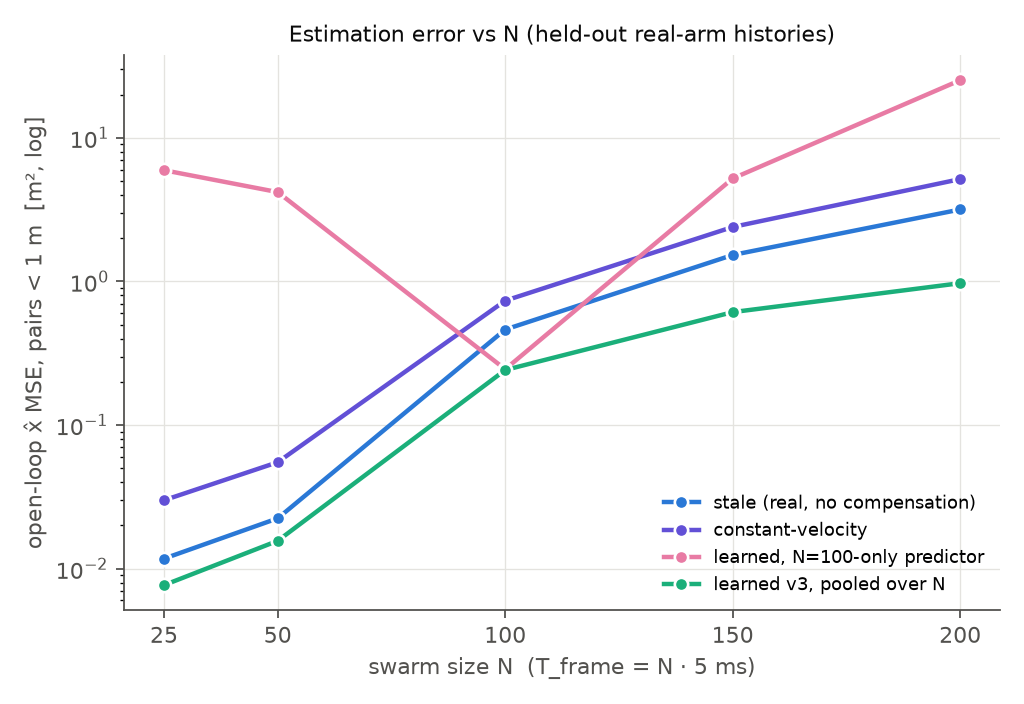
\includegraphics[width=\columnwidth]{fig2_mechanism_openloop.png}
\caption{Open-loop near-pair ($<$1\,m) position MSE on held-out stale-arm histories (Config~G, log scale). A
predictor trained only at $N{=}100$ fails out of distribution; the pooled v3 is below the stale estimate at
every $N$.}
\label{fig:openloop}
% SRC: results/overnight_figures/fig2_mechanism_openloop.png; figure_data.csv fig2_openloop_mse
\end{figure}

\emph{Margin.} With v3 at $N{=}100$ (Config~G), a larger $\dsafe$ lowers ever-collided (0.325, 0.072, 0.020,
0.010 for $\dsafe{=}0.55$, 0.70, 0.85, 1.00) but freezes the swarm (completeness 1.000, 0.958, 0.764,
0.692)\textsuperscript{\dag}; the pre-registered rule selects $\dsafe{=}0.70$. Without compensation the sign
flips: at $N{=}50$ the stale swarm reaches safe success 0.284 with $\dsafe{=}0.55$ but only 0.056 with
0.70\textsuperscript{\dag}. A larger margin on a stale estimate triggers more CBF interventions (0.638 vs
0.454) and more evasive motion, which inflates the very error it was meant to cover; a margin helps only on an
accurate estimate.
% SRC: review_amend23 (118e4bd); review_amend22 Step A "Unexpected" (c24e62f). dag = @T, amend39 stage C pending

%=====================================================================
\section{Results}
\label{sec:results}
%=====================================================================
\subsection{Delay, not density, causes collisions}
\label{sec:barrier}
\emph{Mechanism.} The noise\_only swarm keeps the controller, geometry, start packing and sensor-noise draws of
the delayed arms. Its ever-collided is $0.000$, CI $[0,0]$, at every $N$ up to 200
(Table~\ref{tab:crossover}), although at $N{=}150$ and 200 the swarm \emph{starts} closer than $\dsafe$ (minimum
spacing 0.626 and 0.553\,m) and the CBF is active in 91--95\% of steps. The uncompensated swarm collides at every
$N\ge50$. At these densities, collisions are caused by delay-estimation error, not by packing.
% SRC: review_amend24 (eacfb15); review_amend27 Q1 (2edfe32)

\emph{Staleness barrier.} The stale swarm has safe\_N of \SafeNReal{} and the learned swarm of
\SafeNLearned\Pending. Learned minus real \HeadShort{} at matched margin is \GapFifty, \GapHundred,
\GapOneFifty{} and \GapTwoHundred{} at $N{=}50$, 100, 150, 200\Pending, i.e.\ v3 recovers \RecFifty, \RecHundred,
\RecOneFifty{} and \RecTwoHundred\% of the delay-free minus stale gap. Classical compensators fail in this
regime: cv amplifies broadcast noise (safe 0.000 at $N{=}50$, below the uncompensated 0.284), and the
congestion-blind Smith predictor places phantom neighbours in the gate so the swarm locks up (completeness
0.00--0.05 at $N\ge100$)\textsuperscript{\dag}. The headroom above v3 is \Headroom{} at $N{=}100/150/200$.
\ifpending
Under the settled metric safe\_N can only stay or fall (the collision criterion is unchanged, the completeness one
only stricter), so the stale swarm's safe\_N cannot exceed 25.
\fi
% SRC: gen/numbers.tex <- viz/paper_numbers.py; review_amend27 Q2 + Smith (2edfe32)

\begin{table}[t]
\centering\footnotesize
\setlength{\tabcolsep}{3.2pt}
\caption{$N$ crossover in Config~G ($\Tf{=}N\cdot5$\,ms; learned and delay-removed at $\dsafe{=}0.70$).
Ever-collided is metric-independent.\Pending}
\label{tab:crossover}
% GENERATED by viz/paper_numbers.py (source: legacy) -- do not edit
\begin{tabular}{@{}llccccc@{}}
\toprule
 & $N$ & 25 & 50 & 100 & 150 & 200\\
 & $\Tf$ [s] & 0.125 & 0.25 & 0.5 & 0.75 & 1.0\\
\midrule
\multirow{3}{*}{\rotatebox{90}{\scriptsize ever coll.}} & real, $d$ 0.70 & 0.000 & 0.944 & 1.000 & 1.000 & 1.000\\
 & learned v3 & 0.000 & 0.008 & 0.076 & 0.473 & 0.827\\
 & delay removed & 0.000 & 0.000 & 0.000 & 0.000 & 0.000\\
\midrule
\multirow{4}{*}{\rotatebox{90}{\scriptsize safe@$T$}} & real, $d$ 0.55 & 1.000 & 0.284 & 0.000 & 0.000 & 0.000\\
 & real, $d$ 0.70 & 1.000 & 0.056 & 0.000 & 0.000 & 0.000\\
 & learned v3 & 1.000 & 0.992 & 0.880 & 0.479 & 0.137\\
 & delay removed & 1.000 & 1.000 & 1.000 & 1.000 & 0.968\\
\midrule
\multirow{2}{*}{\rotatebox{90}{\scriptsize compl.@$T$}} & learned v3 & 1.000 & 1.000 & 0.950 & 0.857 & 0.599\\
 & delay removed & 1.000 & 1.000 & 1.000 & 1.000 & 0.968\\
\bottomrule
\end{tabular}

\par\vspace{2pt}{\scriptsize\PendingNote\par}
\end{table}

\begin{figure*}[t]
\centering
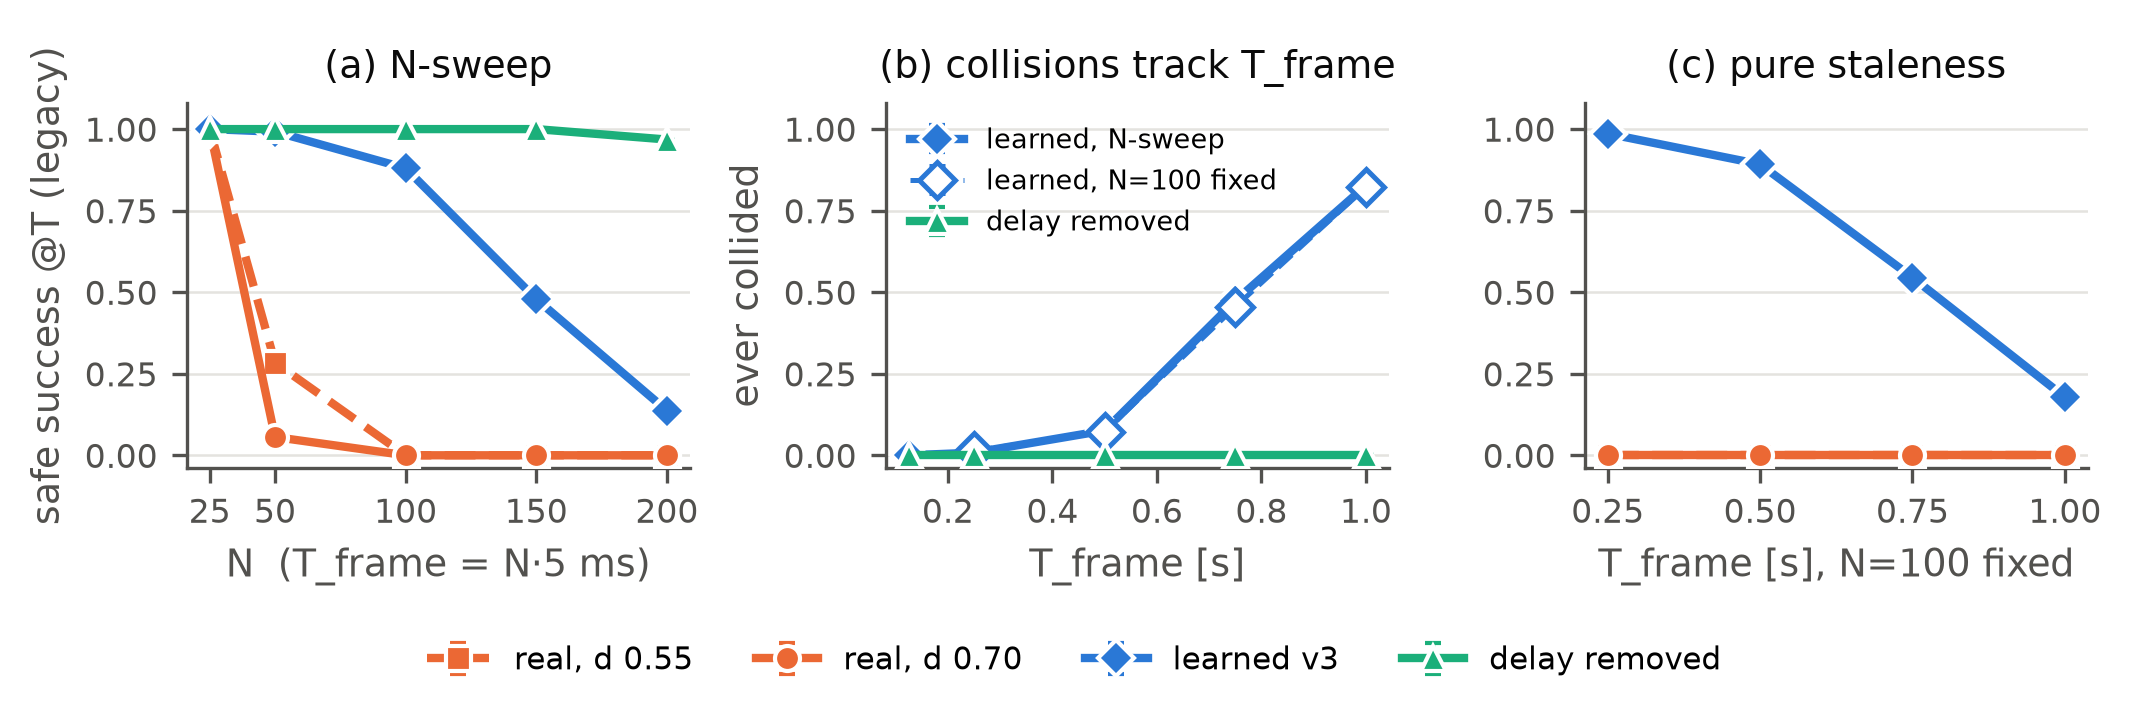
\includegraphics[width=\textwidth]{fig1_staleness.png}
\caption{Staleness, not density. (a)~\HeadMetric{} vs.\ $N$ (Config~G)\Pending. (b)~Learned ever-collided vs.\
$\Tf$ for the $N$-sweep (filled) and for a TDMA-slot sweep at fixed $N{=}100$ (hollow): the curves coincide,
although $N$, packing and neighbour count differ by up to $2\times$; the delay-removed swarm never collides.
(c)~\HeadMetric{} vs.\ $\Tf$ at fixed $N{=}100$\Pending. Error bars: 95\% seed bootstrap, 10 seeds.}
\label{fig:staleness}
% SRC: paper/figs/fig1_staleness.png <- viz/paper_figures.py fig_staleness (amend39 CSV or legacy figure_data.csv)
\end{figure*}

\emph{Pure staleness at fixed $N$.} Holding $N{=}100$, geometry and packing fixed and varying only
$\tslot\in\{2.5,5,7.5,10\}$\,ms ($\Tf\in\{0.25,\dots,1.0\}$\,s), learned \HeadShort{} falls as \TauLearned\Pending;
the stale swarm collides at every $\Tf$, and learned minus real is \TauGap{} (all CIs exclude 0). At equal $\Tf$
the learned ever-collided at fixed $N$ (\TauEverFixed) equals the $N$-sweep value (\TauEverSweep) within CI at all
four points (Fig.~\ref{fig:staleness}b). Learned completeness, in contrast, stays high at fixed $N$
(\TauComplFixed) but falls to \ComplLearnedLargeN{} at $N{=}150/200$\Pending: for the compensated swarm,
\emph{collisions track staleness and completeness tracks density}. For the stale swarm the neighbour count also
matters (ever 1.000 at $N{=}100$, $\Tf{=}0.25$\,s vs 0.944 at $N{=}50$), but it is unsafe either way. Varying
the gate width from 1.5 to 7.0\,m ($4.7\times$ in gate flux) at $N{=}100$ barely moves either arm (learned ever
0.07--0.13; open-loop error ratio flat at 0.52--0.53)\textsuperscript{\dag}.
% SRC: gen/numbers.tex (Tau*); review_amend26 Q3 (ac32b09); review_amend25 (1ce2b21)

\subsection{Compensation helps only through the CBF}
\label{sec:layers}
We feed the compensated (or oracle) estimate to one layer only and the stale estimate to the other
(Fig.~\ref{fig:layers}). In Config~G, compensation fed only to the MFG density term changes safe success by exactly
$0.000$, CI $[0,0]$, at every $N\in\{100,150,200\}$, for both the learned and the oracle estimate; every agent
still collides, so this zero holds under any arrival metric. Fed only to the CBF it recovers 104/105/72\%
(learned) and 100/100/100\% (oracle) of the both-layers gain\textsuperscript{\dag}. In Config~S, recomputed exactly
from stored trajectories, an oracle-clean CBF with a delayed MFG gives $+0.968$\ci{+0.962}{+0.974} safe settled
over the stale swarm, close to full delay removal ($+0.988$); a clean MFG with a delayed CBF gives
$+0.000$\ci{0}{0} (without the band: $+0.802$ and $+0.000$). Collisions are identical under all metrics in all
51 Config~S rollouts.
% SRC: review_amend27 Q3 (2edfe32); results/amend39_configS_band/report.json contrasts (b0.30, b0.00); amend38 A2 identity

\begin{figure*}[t]
\centering
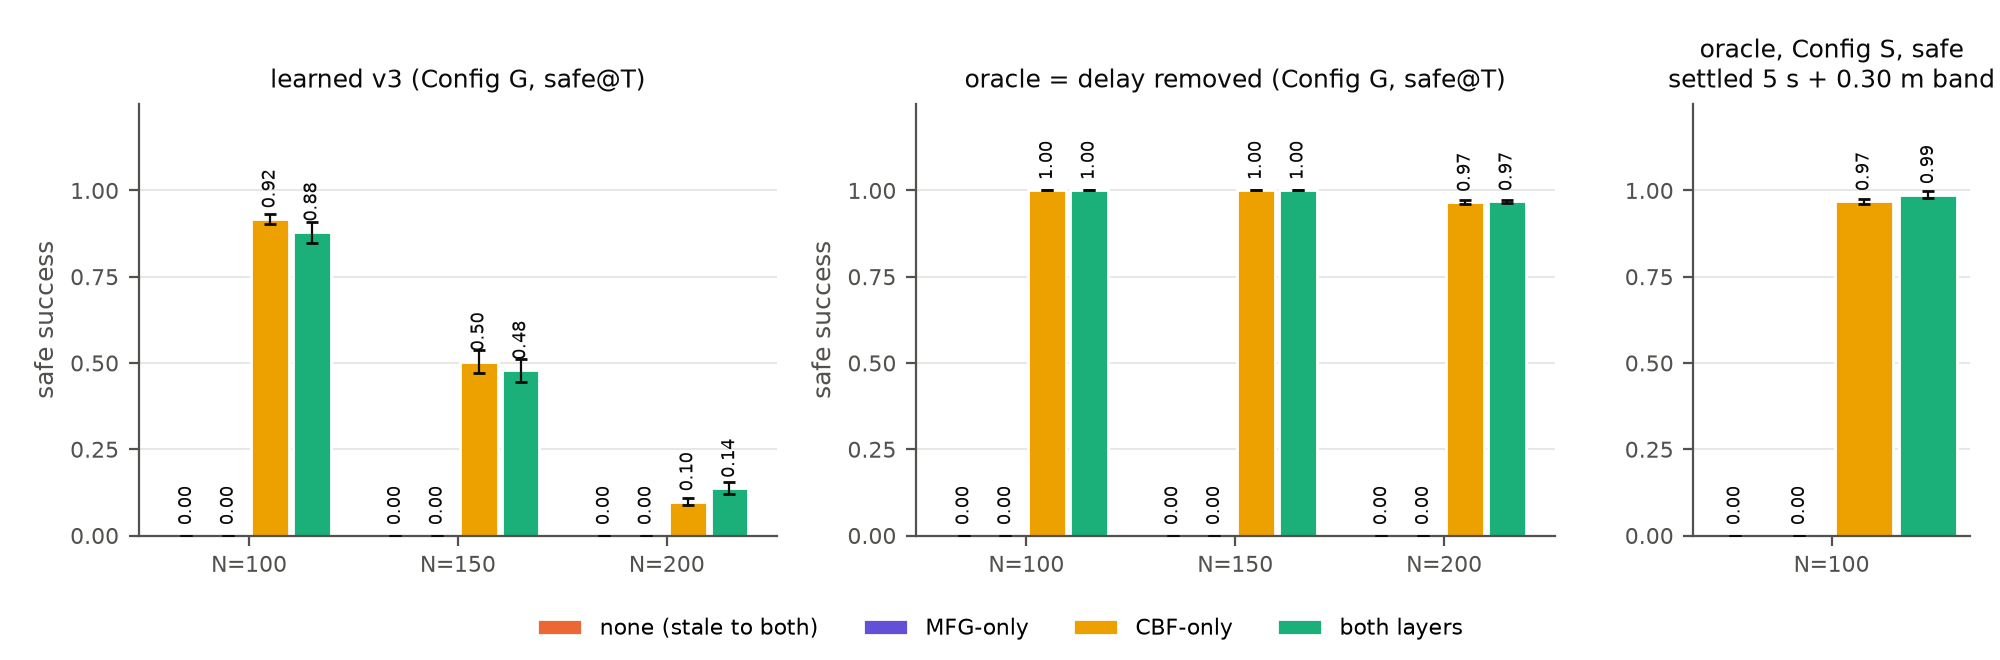
\includegraphics[width=0.92\textwidth]{fig6_layer_split.png}
\caption{Layer split. ``MFG-only'' feeds the compensated (or oracle) estimate to the MFG density term and the
stale one to the CBF; ``CBF-only'' the reverse. Left, centre: Config~G, $\dsafe{=}0.70$, safe@$T$, 10
seeds\textsuperscript{\dag}. Right: Config~S, $N{=}100$, oracle, safe settled with the 0.30\,m band, 5 seeds,
exact. MFG-only equals no compensation (0.000) in every cell.}
\label{fig:layers}
% SRC: viz/paper_figures.py fig_layers <- amend27 report.json, amend39_configS_band report.json
\end{figure*}

\emph{What the MFG layer is for.} With exact positions (Config~S) the full MFG+CBF controller settles 1.000 of the
swarm against 0.650 for a CBF-only controller with decoupled single-agent routing, $+0.350$\ci{+0.310}{+0.400}
($+0.318$ without the band), both with zero collisions. CBF-only agents are frozen outside the goal, not
oscillating: their success is identical at every window. Conversely, the MFG without the CBF arrives
(completeness 1.000) but 99.8\% of agents collide. Learned minus real in Config~S is $+0.186$\ci{+0.134}{+0.248}
($+0.154$ without the band), with a different, $N{=}100$-only predictor.
% SRC: amend39_configS_band report.json arms fresh/fresh_nomfg/fresh_nocbf + contrasts; review_amend37 (window-invariant)

\subsection{Why settled arrival with a band}
\label{sec:metric}
Scoring arrival at the final instant $T$ overstates completeness: a controller can rush stragglers in at the last
moment (with an MFG terminal cost, 14--18 agents were still outside 1\,s before $T$ yet counted as arrived), and in
the delayed arms almost half the agents counted at $T$ churn in and out of the disc (real 0.718 at $T$ vs 0.426
settled, $b{=}0$). Requiring settled arrival removes both effects. Without a band, however, even the delay-free
swarm settles only 0.920 (exact positions) and 0.800 (with sensor noise). A diagnosis of every non-settler shows a
ring on the rim, not stuck agents (Fig.~\ref{fig:rim}): all exact-position non-settlers end within 0.30\,m of the
goal boundary (median 0.18\,m outside); 50\% oscillate across it and 30\% rest where goal attraction and
crowd aversion balance; with sensor noise, noise-widened CBF spacing makes the outer ring jitter. The 0.30\,m band
(one collision distance) counts this ring: delay-free safe settled becomes 1.000 and 0.988. Collision metrics
are unaffected by either choice.
% SRC: review_amend36 (last-second inflow); review_amend38 A2 + B; amend39_configS_band arms fresh/noise_only

\begin{figure}[t]
\centering
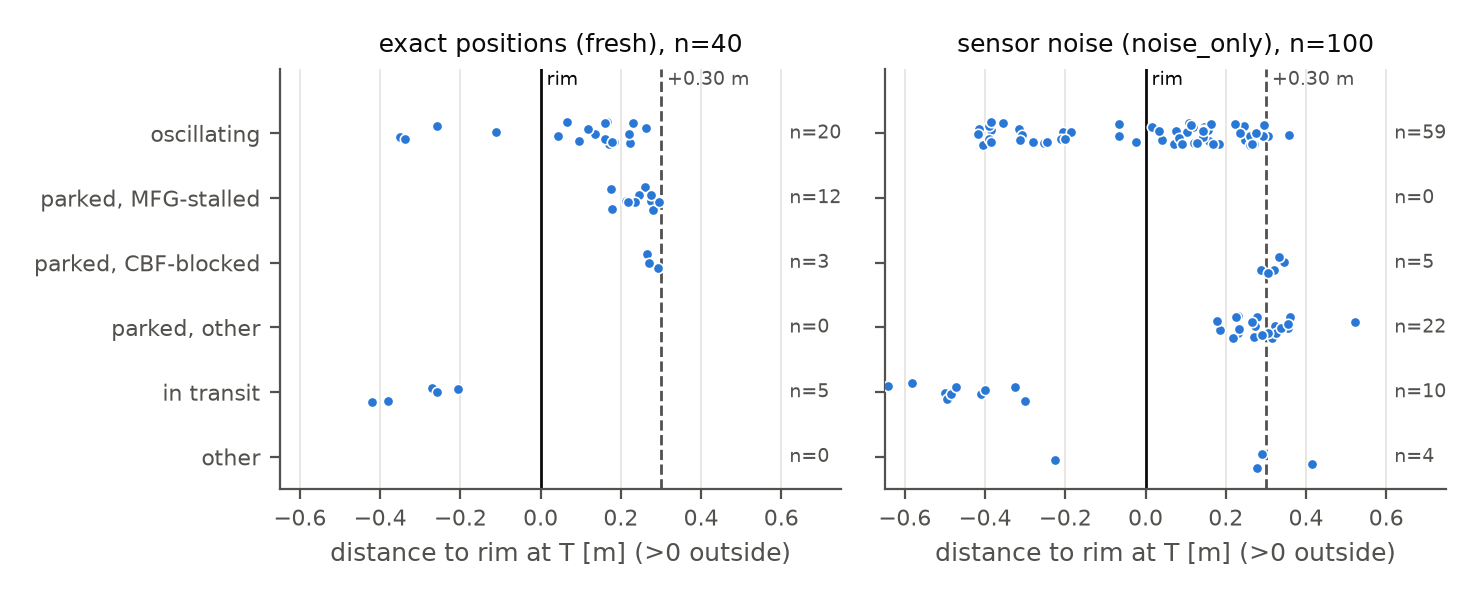
\includegraphics[width=\columnwidth]{fig7_rim_nonsettlers.png}
\caption{Delay-free non-settlers (Config~S, $b{=}0$, 5 seeds): distance to the goal rim at $T$ by behaviour class.
All exact-position non-settlers lie within the 0.30\,m band (dashed).}
\label{fig:rim}
% SRC: viz/paper_figures.py fig_rim <- amend38 report.json B
\end{figure}

\subsection{A calibrated uncertainty margin does not replace compensation}
\label{sec:sigma}
We replaced the constant margin by a per-neighbour one, $\dsafe^{ij}=\max(0.70,\,D_{\mathrm{c}}+q_\alpha\sigma_{ij})$,
where $\sigma_{ij}$ is a learned model of v3's error and $q_\alpha$ an $(N,\sigma)$-binned split-conformal quantile;
every gate was fixed before its data existed. The error model \emph{ranks} risk well (top-10\% errors found with
AUC 0.78--0.86 per $N$) but does not \emph{size} it (pooled $R^2_{\log}{=}0.35$, negative within the top decile).
Offline coverage at $\alpha{=}0.05$ is 0.955. In closed loop, with the margin capped at 1.5\,m, the primary arm
beats the best constant margin by $+0.039$\ci{+0.005}{+0.075} safe@$T$ at $N{=}150$ but loses by
$-0.189$\ci{-0.200}{-0.177} at $N{=}200$, where every agent collides in every $\sigma$ arm: the registered win
criterion is not met. Coverage falls to 0.77 on near pairs and 0.69 where the margin binds at $N{=}200$, because the
controller that consumes the margin shifts the distribution it was calibrated on. A plausible, untested reading:
at $N{=}150$ the margin binds on 12.6\% of CBF rows and protects a few risky pairs; at $N{=}200$ it binds on 75.2\%
and acts as a broad, large margin on out-of-calibration estimates, the regime in which a larger margin hurts
(Sec.~\ref{sec:method}). A fixed margin on top of accurate compensation remains the pragmatic recipe.
% SRC: review_gpred (01701ef); review_amend31 G-cal; review_amend35 G-win + closed-loop coverage (14049bb); amend35 report.json sigma_bind_frac

%=====================================================================
\section{Limitations}
\label{sec:limits}
%=====================================================================
\emph{No hard guarantee.} The CBF certifies separation of \emph{estimated} positions. No margin we tested is both
collision-free and complete at $N\ge100$ with the learned predictor; at $N\ge150$ most of the gap remains.
\emph{Scope.} One single-gate scenario (two parameterizations), single-integrator agents, simulated perception,
offline MFG solved per $N$. \emph{Baselines.} cv and Smith fail for identifiable reasons; a noise-optimal
least-squares fit on the learned arm's four-broadcast window was specified but not run, so ``learned beats
classical'' is stated against these two only. \emph{Statistics.} Config~S has 5 seeds (a paired sign-flip test
cannot reach $p<0.05$); the learned GPU path is not bit-deterministic across runs (the $N{=}100$ cell replicated
as 0.892 vs 0.880, within CI). \emph{Metric.} The settled metric and band were adopted after @$T$ results were seen;
we report $b{=}0$ next to every banded number.
% SRC: review_amend23 C/E; review_amend27 "Fairness consequence"; prereg amend32 (not run); review_amend34; review_amend23 B.1

%=====================================================================
\section{Conclusion}
%=====================================================================
In a two-layer MFG+CBF swarm with drone-sized keep-out distances, UWB/vision noise and TDMA delay, collisions are
caused by stale neighbour estimates, not by density: removing the delay removes every collision up to $N{=}200$,
and a pure-staleness sweep reproduces the collision rate of the $N$-sweep. Compensation belongs in the CBF layer; fed
to the MFG density term it is worth exactly zero, even as an oracle, while the MFG layer earns its place through
liveness. A conformally calibrated uncertainty margin does not move the constant-margin frontier, and its coverage
breaks in closed loop. Recovering safety at large staleness therefore requires acting \emph{before} the reactive
filter, for example by limiting closing speed under perception uncertainty, routing that avoids fast-closing
configurations, or allocating TDMA slots to closing pairs.

\section*{Reproducibility Statement}
All code (MFG solver, rollout, perception and TDMA model, CBF-QP, predictor training, analysis and figure
scripts), the frozen predictor weights (SHA-256 \texttt{9583cb7c\ldots}), every pre-registered analysis plan with
its hash, the per-seed result files and the raw trajectories of the headline cells (with a SHA-256 manifest) will
be released upon acceptance at \url{https://github.com/<to-be-released>}. Each reported cell names its
configuration file and seeds (0--9 in Config~G, 0--4 in Config~S). Config~G ran on single NVIDIA A100-80GB GPUs
(the capped $\sigma$-CBF comparison on an RTX PRO 6000, with all its comparators re-run on that GPU), Config~S on
CPU, with JAX at \texttt{matmul\_precision=highest}. Table~\ref{tab:crossover}, Fig.~\ref{fig:staleness} and the
macro numbers in the text are generated by script from the result files. Confidence intervals are 95\% seed-level
bootstrap with $10^4$ resamples. The learned-arm GPU path is not bit-deterministic across runs; replicates agree
within CI.

\bibliographystyle{IEEEtran}
\bibliography{refs}

\end{document}
